% LaTeX document embedding the architecture diagram and expanded descriptions
\documentclass[11pt]{article}
\usepackage[a4paper,margin=1in]{geometry}
\usepackage{graphicx}
\usepackage{hyperref}
\usepackage{listings}
\usepackage{courier}
\lstset{basicstyle=\footnotesize\ttfamily,breaklines=true}
\title{middleware-dt: Architecture and Component Details}
\author{Digital-Twins-RSBR}
\date{\today}

\begin{document}
\maketitle

\begin{figure}[ht]
  \centering
  % Ensure the PNG was generated by Graphviz: docs/architecture_diagram.png
  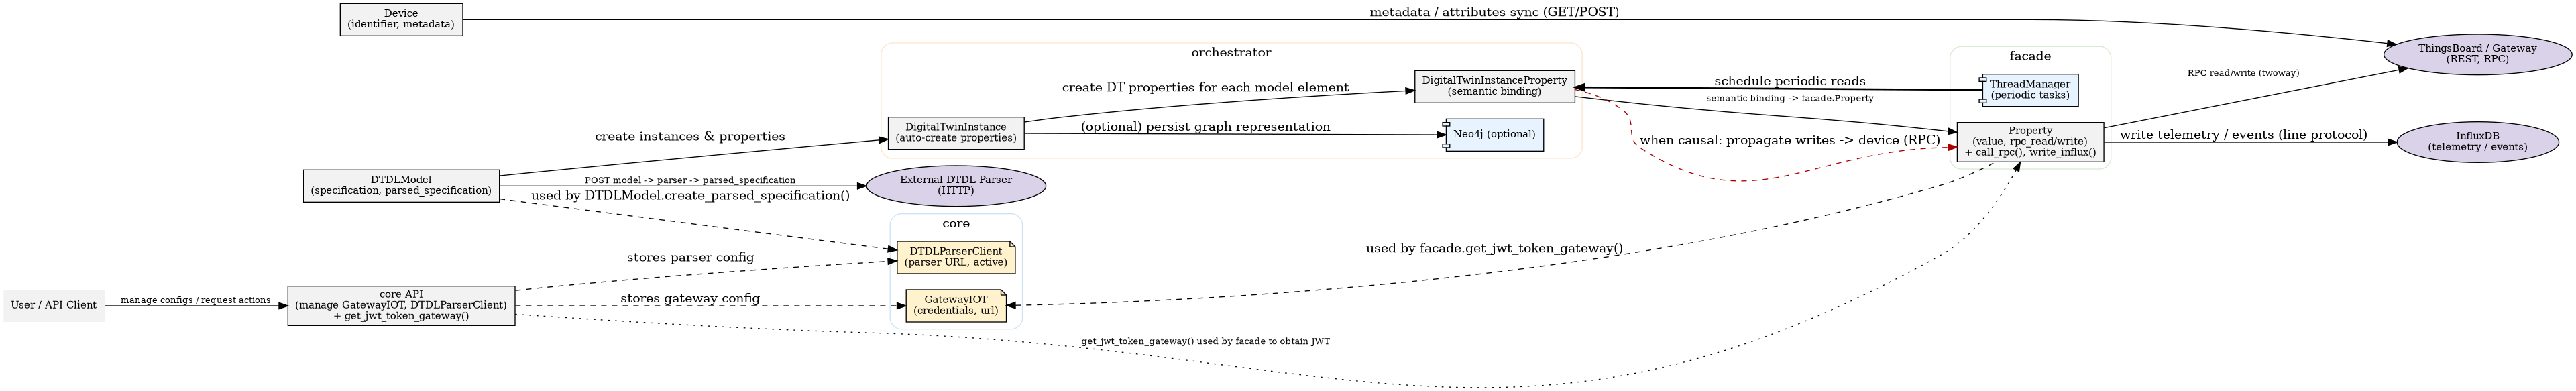
\includegraphics[width=0.95\textwidth]{docs/architecture_diagram.png}
  \caption{High-level architecture of middleware-dt. The three main modules are \texttt{core}, \texttt{facade} and \texttt{orchestrator}.}
\end{figure}

\section{Overview}
The system is organized in three main modules.
\begin{itemize}
  \item \textbf{core}: configuration and small API endpoints (gateway and DTDL parser clients, token helpers).
  \item \textbf{facade}: adapter layer to gateways (e.g., ThingsBoard) and devices; it handles RPCs, telemetry collection and writes to InfluxDB.
  \item \textbf{orchestrator}: DTDL model ingestion, instance creation, semantic binding between digital twin properties and real devices, and optional graph persistence.
\end{itemize}

\section{core}
\subsection*{Responsibilities}
Store gateway configuration and available DTDL parser clients; provide a helper to fetch JWT tokens for gateways.

\subsection*{Representative code}
\begin{lstlisting}
# get_jwt_token_gateway(gateway_id)
response = requests.post(
  f"{gateway.url}/api/auth/login",
  json={"username": gateway.username, "password": gateway.password}
)
if response.status_code == 200:
  token = response.json().get('token')
\end{lstlisting}

\section{facade}
\subsection*{Responsibilities}
Model devices and properties, synchronize shared attributes and labels from ThingsBoard, issue RPCs (read/write), and write telemetry/events to InfluxDB. Also provide a small thread manager to schedule periodic reads.

\subsection*{Property write sequence (summary)}
\begin{enumerate}
  \item Application requests a write to a property or a DT causal property is updated.
  \item `Property.save()` calls `Property.call_rpc(RPCCallTypes.WRITE)`.
  \item A JWT is obtained and a two-way RPC is posted to the gateway. A sent timestamp is written to InfluxDB (best-effort).
  \item If the RPC returns a value, the local `Property.value` is updated and, if configured, written to InfluxDB.
\end{enumerate}

\subsection*{Representative code}
\begin{lstlisting}
session = get_session_for_gateway(gateway.id)
response = session.post(
    f"{gateway.url}/api/rpc/twoway/{device.identifier}",
    json={"method": prop.rpc_write_method, "params": prop.get_value()},
    headers=headers, timeout=8
)
\end{lstlisting}

\section{orchestrator}
\subsection*{Responsibilities}
Persist DTDL models and parsed representations, create model elements/relationships, create hierarchical digital twin instances and properties, execute semantic binding using sentence embeddings, and optionally persist a Neo4j graph.

\subsection*{DTDL parsing and model materialization}
A `DTDLModel` sends the `specification` to an external DTDL parser service and stores the `parsed_specification`. Then, it materializes `ModelElement` and `ModelRelationship` rows so that instances can be created.

\subsection*{Semantic binding (short)}
Embeddings for textual contexts are computed with a sentence transformer (e.g., \texttt{all-MiniLM-L6-v2}). Cosine similarity is used to find the best candidate device property. The system uses a conservative acceptance threshold (0.60) and leaves ambiguous matches for human inspection.

\section{Contracts and failure modes}
\begin{itemize}
  \item DTDL parser unavailable $
ightarrow$ parsing fails and must be retried.
  \item Gateway JWT failures $
ightarrow$ facade logs and upper layers must handle unreachable devices.
  \item RPC timeouts $
ightarrow$ pseudo-responses with status 503/504 are returned internally for deterministic handling.
\end{itemize}

\section{Suggested experiments for the article}
\begin{itemize}
  \item Measure RPC latency and success rate across varying network conditions and gateway loads.
  \item Evaluate semantic binding accuracy on an annotated dataset (precision/recall) and report human correction rates.
  \item Compare InfluxDB write latency and ingestion throughput against telemetry volume.
\end{itemize}

\section{Appendix: short code examples}
See `docs/architecture_expanded.md` for the same fragments with additional commentary.

\end{document}
